\documentclass[a4paper, 11pt]{article}
\usepackage{listings}
\usepackage{amsmath}
\usepackage{fullpage}
\usepackage{comment}
\newcommand{\argmax}{\operatornamewithlimits{arg\,max}}
\newcommand{\argmin}{\operatornamewithlimits{arg\,min}}
\lstset{
	tabsize=2,
	basicstyle=\footnotesize\ttfamily,
	%numbers=left,
	%numberstyle=\footnotesize,
	%xleftmargin=0.05\textwidth,
% 	language = Java,
	keywordstyle =\bfseries \color{blue},
	commentstyle =\color{green},
	stringstyle =\itshape \color{red}
}

\usepackage{graphicx}
\usepackage{wrapfig}
\usepackage[
	colorlinks=true,
	urlcolor=black,
	linkcolor=blue,
	citecolor = black,
	naturalnames=true,
	pdftitle={LIMES},
	pdfsubject={Manual},
	pdfauthor={Axel Ngonga},
	pdfkeywords={LIMES, Link Discovery, Linked Data, Machine Learning, framework, Linked Data, SPARQL}
]{hyperref}
%%%%%%%%%%%%%%%%%%%%%%%%%%%%%%%%%%%%%%%%%%%%%%%
\begin{document}
\thispagestyle{empty}
% titlepage
\begin{titlepage}
\begin{center}
% Upper part of the page

\includegraphics[width=\textwidth]{images/limes_logo.pdf}

% Title
% \bfseries
\centering
\Huge User Manual

\huge Version 0.6.RC4
%\begin{minipage}{0.7\textwidth}
%	\begin{flushleft} 
%		\large{
%		Axel-Cyrille Ngonga Ngomo\\
%				Johanisgasse 26\\
%				Room 5-22\\
%				04103 Leipzig\\
%				ngonga@informatik.uni-leipzig.de}
%	\end{flushleft}
%\end{minipage}\\
	
\vfill
% Bottom of the page
{\large \today}
\end{center}
\end{titlepage}
\tableofcontents
%%%%%%%%%%%%%%%%%%%%%%%%%%%%%%%%%%%%%%%%%%%%%%%

\newpage
\section{Introduction}
LIMES, the \textbf{Li}nk Discovery Framework for \textbf{Me}tric \textbf{S}paces, is a framework for discovering links between entities contained in Linked Data sources. LIMES is a hybrid framework that combines the mathematical characteristics of metric spaces as well prefix-, suffix- and position filtering to compute pessimistic approximations of the similarity of instances. These approximations are then used to filter out a large amount of those instance pairs that do not suffice the mapping conditions. By these means, LIMES can reduce the number of comparisons needed during the mapping process by several orders of magnitude and complexity without loosing a single link.  
%Thus, it is more time-efficient than current frameworks for Link Discovery. Still, it achieves exactly the same results as brute appproaches (i.e., 100\% of their precision and recall) because of the type of approximations it uses. 

		\begin{figure}[ht!]
			\centering
			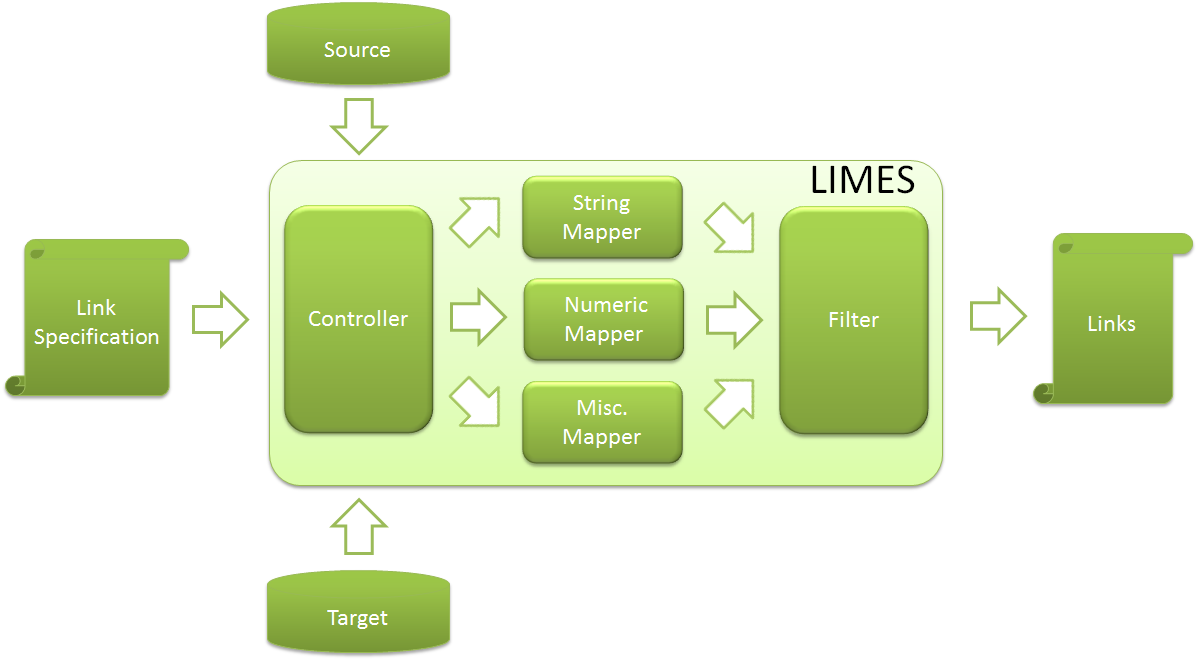
\includegraphics[width = 0.95\textwidth]{images/workflow.png}
			\caption{General Workflow of LIMES}
			\label{fig:workflow}
		\end{figure}

The general workflow implemented by the LIMES framework is depicted in Figure~\ref{fig:workflow}.
Given the source $S$, the target $T$ and a link specification, LIMES first separates the different data types to merge. 
Strings are processed by using suffix-, prefix- and position filtering in the string mapper.
Numeric values (and all values that can be mapped efficiently to a vector space) are mapped to a metric space and processed by the HYPPO algorithm.
All other values are mapped by using the miscellaneous mapper.
The results of all mappers processing are filtered and merged by using time-efficient set and filtering operations.

The advantages of LIMES' approach are manifold. 
First, it implements \textbf{highly time-optimized} mappers, making it a complexity class faster than other Link Discovery Frameworks. Thus, the larger the problem, the faster LIMES is w.r.t. other Link Discovery Frameworks. In addition, \textbf{LIMES is guaranteed to lead to exactly the same matching as a brute force approach while at the same time reducing significantly the number of comparisons}. In addition, LIMES supports a \textbf{large number of input and output formats} and can be extended very easily to fit new algorithms , new datatypes, new preprocessing functions and others thank to its modular architecture displayed in Figure \ref{fig:architecture}.

\begin{figure}[ht!]
			\centering
			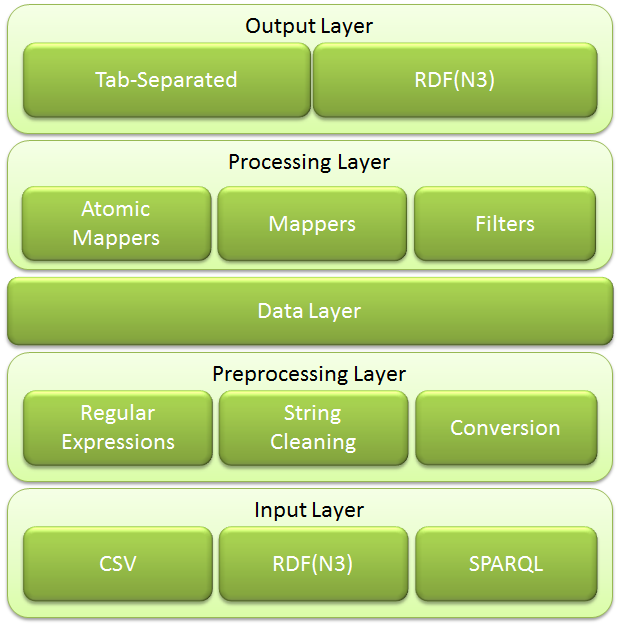
\includegraphics[width = 0.6\textwidth]{images/architecture.png}
			\caption{Architecture of LIMES}
			\label{fig:architecture}
		\end{figure}
		
In general, LIMES can be used to set links between two data sources, e.g., a novel data source created by a data publisher and existing data source such as DBpedia\footnote{\url{http://dbpedia.org}}. This functionality can also be used to detect duplicates within one data source for knowledge curation. The only requirement to carry out these tasks is a simple XML-based configuration file. The purpose of this manual is to explicate the LIMES Configuration Language (LCL) that underlies these configuration files, so as allow users to generate their own configurations. An online version of LIMES is available online at $\texttt{http://limes.aksw.org}$.

\section{Components of a LIMES Configuration File}
A LIMES configuration file consists of ten parts, of which some are optional:
\begin{enumerate}
\item Metadata
\item Prefixes
\item Source data source
\item Target data source
\item Metric for similarity measurement
\item Acceptance condition
\item Review condition 
\item Execution mode (optional)
\item Granularity (optional)
\item Output format
\end{enumerate}
In the following, we will explicate these components by showing successively how LIMES can be configured to compute a mapping between diseases contained in Bio2RDF and LinkedCT.
\subsection{Metadata}
The metadata for a LIMES config file always consists of the following bits of XML:

\begin{ttfamily}
\begin{lstlisting}[language=XML,basicstyle=\scriptsize,numberstyle=\tiny]
<?xml version="1.0" encoding="UTF-8"?>
<!DOCTYPE LIMES SYSTEM "limes.dtd">
<LIMES>
\end{lstlisting}
\end{ttfamily}

\subsection{Prefixes}
Defining a prefix in a LIMES file demands setting two values: the namespace that will be addresses by the prefix and the prefix per se, as shown below. 
\begin{ttfamily}
\begin{lstlisting}[language=XML,basicstyle=\scriptsize,numberstyle=\tiny]
<PREFIX>
		<NAMESPACE>http://www.w3.org/1999/02/22-rdf-syntax-ns#</NAMESPACE>
		<LABEL>rdf</LABEL>
</PREFIX>
\end{lstlisting}
\end{ttfamily}
Here, we set the prefix \texttt{rdf} to correspond to \texttt{http://www.w3.org/1999/02/22-rdf-syntax-ns\#}. A LIMES link specification can contain as many prefixes as required.

\subsection{Source Data Source}
LIMES computes links between items contained in two Linked Data sources dubbed source and target. An example of a configuration for a source data source is shown below.
\begin{ttfamily}
\begin{lstlisting}[language=XML,basicstyle=\scriptsize,numberstyle=\tiny]
<SOURCE>
	<ID>mesh</ID>
	<ENDPOINT>http://mesh.bio2rdf.org/sparql</ENDPOINT>
	<VAR>?y</VAR>
	<PAGESIZE>5000</PAGESIZE>
	<RESTRICTION>?y rdf:type meshr:Concept</RESTRICTION>
	<PROPERTY>dc:title</PROPERTY>
	<TYPE>sparql</TYPE>
</SOURCE>
\end{lstlisting}
\end{ttfamily}

Six properties need to be set. 
\begin{enumerate}
\item Each data source must be given an ID via the tag \texttt{ID}.
\item The SPARQL endpoint of the data source needs to be explicated via the \texttt{ENDPOINT} tag. In case local files (CSV, N3, TURTLE, etc.) are to be linked, \texttt{ENDPOINT} should be set to the absolute path of the file containing the data to link.
\item The variable associated with this endpoint must be specified. This is done by setting the \texttt{VAR} tag. This variable is used later when specifying the metric used to compare the entities retrieved from the source and target endpoints.
\item The fourth property is set via the \texttt{PAGESIZE} tag. This property must be set to the maximal number of triples returned by the SPARQL endpoint to address. For example, the DBpedia endpoint at \url{http://dbpedia.org/sparql} returns a maximum of 1000 triples for each query. LIMES' SPARQL module can still retrieve all relevant instances for the mapping if given this value. If the SPARQL endpoint does not limit the number of triple it returns or if the input is a file, the value of \texttt{PAGESIZE} should be set to -1. 
\item The restrictions of the data to retrieved can be set via the \texttt{RESTRICTION} tag. This tag allows to limit the entries that are retrieved the LIMES' query module. In this particular example, we only instances of MESH concepts. 
\item The \texttt{PROPERTY} tag allows to specify the properties that will be used during the linking. It is important to note that the property tagcan also be used to specify the preprocessing on the input data. For example, setting \texttt{rdfs:label AS nolang}, one can ensure that the language tags get removed from each \texttt{rdfs:label} before it is written in the cache. Pre-processing functions can be piped into one another by using \texttt{->}. For example, \texttt{rdfs:label AS nolang->lowercase} will compute \texttt{lowercase(nolang(rdfs:label))}.
\end{enumerate}

 The pre-processing functions include: 
\begin{itemize}
\item \texttt{nolang} for removing language tags, 
\item \texttt{lowercase} for converting the input string into lower case,  
\item \texttt{uppercase} for converting the input string into upper case, 
\item \texttt{number} for ensuring that only the numeric characters, ``.'' and ``,'' are contained in the input string,
\item \texttt{replace(String a,String b)} for replacing each occurrence of \texttt{a} with \texttt{b},
\item \texttt{cleaniri} for removing all the prefixes from IRIs,
\item \texttt{celsius} for converting Fahrenheit to Celsius,
\item \texttt{fahrenheit} for converting Celsius to Fahrenheit.
\end{itemize}

Sometimes, generating the right link specification might either require merging property values (for example, the \texttt{dc:title} and \texttt{foaf:name} of MESH concepts) or splitting property values (for example, comparing the label and \texttt{foaf:homepage} of source instances and the \texttt{foaf:homepage} of target instances as well as \texttt{foaf:homepage AS cleaniri} of the target instances with the \texttt{rdfs:label} of target instances. To enable this goal, LIMES provides the \texttt{RENAME} operator which simply store either the values of a property or the results of a preprocessing into a different property field. For example, \texttt{foaf:homepage AS cleaniri RENAME label} would stored the homepage of a object without all the prefixes in the name property. The user could then access this value during the specification of the similarity measure for comparing sources and target instances. Note that the same property value can be used several times. Thus, the following specification fragment is valid and leads to the the \texttt{dc:title} and \texttt{foaf:name} of individuals)  of MESH concepts being first cast down to the lowercase and then merged to a single property.

\begin{ttfamily}
\begin{lstlisting}[language=XML,basicstyle=\scriptsize,numberstyle=\tiny]
<SOURCE>
	<ID>mesh</ID>
	<ENDPOINT>http://mesh.bio2rdf.org/sparql</ENDPOINT>
	<VAR>?y</VAR>
	<PAGESIZE>5000</PAGESIZE>
	<RESTRICTION>?y rdf:type meshr:Concept</RESTRICTION>
	<PROPERTY>dc:title AS lowercase RENAME name</PROPERTY>
	<PROPERTY>foaf:name AS lowercase RENAME name</PROPERTY>
	<TYPE>sparql</TYPE>
</SOURCE>
\end{lstlisting}
\end{ttfamily}

In addition, the following allows splitting the values of \texttt{foaf:homepage} into the property values \texttt{name} and \texttt{homepage}.

\begin{ttfamily}
\begin{lstlisting}[language=XML,basicstyle=\scriptsize,numberstyle=\tiny]
<SOURCE>
	<ID>mesh</ID>
	<ENDPOINT>http://mesh.bio2rdf.org/sparql</ENDPOINT>
	<VAR>?y</VAR>
	<PAGESIZE>5000</PAGESIZE>
	<RESTRICTION>?y rdf:type meshr:Concept</RESTRICTION>
	<PROPERTY>foaf:homepage AS lowercase RENAME homepage</PROPERTY>
	<PROPERTY>foaf:homepage AS cleaniri->lowercase RENAME name</PROPERTY>
	<TYPE>sparql</TYPE>
</SOURCE>
\end{lstlisting}
\end{ttfamily}

In addition, a source type can be set via \texttt{TYPE}. The default type is set to \texttt{SPARQL} (for a SPARQL endpoint) but LIMES also supports reading files directly from the harddrive. The supported data formats are
\begin{itemize}
\item \texttt{CSV}: Character-separated file can be loaded directly into LIMES. Note that the separation character is set to \texttt{TAB} as a default. The user can alter this setting programmatically. 
\item \texttt{N3} (which also reads \texttt{NT} files) reads files in the \texttt{N3} language.
\item \texttt{N-TRIPLE} reads files in W3C's core N-Triples format.\footnote{\url{http://www.w3.org/TR/rdf-testcases/\#ntriples}}
\item  \texttt{TURTLE} allows reading files in the \texttt{Turtle} syntax.\footnote{\url{http://www.w3.org/TR/turtle/}}
\end{itemize}
Consequently, if you want to download data from a SPARQL endpoint, there is no need to set the \texttt{<TYPE>} tag. 
If instead you want to read the source (or target) data from a file, the \texttt{<ENDPOINT>} tag should contain the path to the file to read, e.g. \texttt{<ENDPOINT>C:/Files/dbpedia.nt</ENDPOINT>}
In addition, the \texttt{<TYPE>} tag then needs to be set, for example by writing \texttt{<TYPE>NT</TYPE>}.
\subsection{Target Data Source}
Configuring the target data source is very similar to configuring the source data source. The only difference lies in the beginning tag, i.e., \texttt{TARGET} instead of \texttt{SOURCE}. In the example shown below, we retrieve the \texttt{condition\_name} of a condition from LinkedCT. We do no set the type of the source. Thus, LIMES supposes it is a SPARQL endpoint.

\begin{ttfamily}
\begin{lstlisting}[language=XML,basicstyle=\scriptsize,numberstyle=\tiny]
<TARGET>
	<ID>linkedct</ID>
	<ENDPOINT>http://data.linkedct.org/sparql</ENDPOINT>
	<VAR>?x</VAR>
	<PAGESIZE>5000</PAGESIZE>
	<RESTRICTION>?x rdf:type linkedct:condition</RESTRICTION>
	<PROPERTY>linkedct:condition_name</PROPERTY>
</TARGET>
\end{lstlisting}
\end{ttfamily}

\subsection{Metric Expression for Similarity Measurement}
One of the core improvements of the newest LIMES kernels is the provision of a highly flexible language for the specification of complex metrics for linking (set by using the \texttt{METRIC} tag as exemplified below).

\begin{ttfamily}
\begin{lstlisting}[language=XML,basicstyle=\scriptsize,numberstyle=\tiny]
<METRIC>
trigrams(y.dc:title, x.linkedct:condition_name)
</METRIC>
\end{lstlisting}
\end{ttfamily}

In this example, we use the Trigrams metric to compare the \texttt{dc:title} of the instances retrieved from the source data source, with which the variable \texttt{y} is associated, with the \texttt{linkedct:}\\\texttt{condition\_name} of the instances retrieved from the target data source, with which the variable \texttt{x} is associated. While such simple metrics can be used in many cases, complex metrics are necessary in complex linking cases. LIMES includes a formal grammar for specifying complex configurations of arbitrary complexity. For this purpose, two categories of binary operations are supported: Metric operations and boolean operations.

\textbf{Metric operations} allow to combine metric values. They include the operators \texttt{MIN}, \texttt{MAX}, \texttt{ADD} and \texttt{MULT}, e.g. as follows:

\begin{ttfamily}
\begin{lstlisting}[language=XML,basicstyle=\scriptsize,numberstyle=\tiny]
MAX(trigrams(x.rdfs:label,y.dc:title),euclidean(x.lat|long, y.latitude|longitude)).
\end{lstlisting}
\end{ttfamily}

This specification computes the maximum of (1) the trigram similarity of x's \texttt{rdfs:label} and y's \texttt{dc:title} and (2) the 2-dimension euclidean distance of x's \texttt{lat} and \texttt{long} mit y's \texttt{latitude} and \texttt{longitude}, i.e., 

$\sqrt{(x.lat- y.latitude)^2 + (x.long - y.longitude)^2}$. 

Note that euclidean supports arbitrarily many dimensions. In addition, note that \texttt{ADD} allows to define weighted sums as follows:

\begin{ttfamily}
\begin{lstlisting}[language=XML,basicstyle=\scriptsize,numberstyle=\tiny]
ADD(0.3*trigrams(x.rdfs:label,y.dc:title), 
    0.7*euclidean(x.lat|x.long, y.latitude|y.longitude)).
\end{lstlisting}
\end{ttfamily}

\textbf{Boolean operations} allow to combine and filter the results of metric operations and include \texttt{AND}, \texttt{OR}, \texttt{DIFF}, e.g. as follows:

\begin{ttfamily}
\begin{lstlisting}[language=XML,basicstyle=\scriptsize,numberstyle=\tiny]
AND(trigrams(x.rdfs:label,y.dc:title)|0.9,
    euclidean(x.lat|x.long, y.latitude|y.longitude)|0.7).
\end{lstlisting}
\end{ttfamily}

This specification returns all links such that (1) the trigram similarity of x's \texttt{rdfs:label} and y's \texttt{dc:title} is greater or equal to 0.9 and (2) the 2-dimension euclidean distance of x's \texttt{lat} and \texttt{long} mit y's \texttt{latitude} and \texttt{longitude} is greater or equal to 0.7.

The current version of LIMES supports the string metrics 
\begin{itemize}
\item \texttt{Trigrams},
\item \texttt{Cosine},
\item \texttt{Jaccard}, 
\item \texttt{Levenshtein},
\item \texttt{Jaro} and
\item \texttt{Jaro-Winkler}
\end{itemize}
\texttt{Overlap} as well as \texttt{Monge-Elkan} are currently being added.
In addition it supports comparing numeric vectors by using the 
\begin{itemize}
\item \texttt{Euclidean} metric as well as 
\item the \texttt{Orthodromic} distance.
\end{itemize}
While the Euclidean measure can deal with n-dimensional data, the orthodromic distance assumes that it is given a WKT POINT as input.
If the input is a polygon, it uses the Hausdorff distance.
The similarity between polygons can be measured by using the 
\begin{itemize}
\item \texttt{Hausdorff} distance,
\item \texttt{Sum of minimums} distance,
\item \texttt{Fréchet} distance,
\item \texttt{Fair surjection},
\item \texttt{Surjection} and 
\item \texttt{SymmetricHausdorff} distance.
\end{itemize}
Currently, these distances can deal with POLYGON and LINESTRING. 
More complex distance measures are being added.
%
%\subsection{Number of exemplars}
%The user can choose to set the number of exemplars to be used by LIMES manually. This setting can be carried out as shown below.
%\begin{verbatim}
%<EXEMPLARS> 70 </EXEMPLARS>
%\end{verbatim}
%In this example, the number of exemplars is set to 70. It is important to notice that this setting is optional. If not set, LIMES uses the value  $\lfloor{\sqrt{|T|}}\rfloor$ for the number of exemplars, where $T$ is the target knowledge source for the matching task.

\subsection{Acceptance Condition}
Setting the acceptance condition basically consists of setting the value for the threshold above which links are considered to be valid and not to required further curation. This can be carried out as exemplified below.
\begin{ttfamily}
\begin{lstlisting}[language=XML,basicstyle=\scriptsize,numberstyle=\tiny]
<ACCEPTANCE>
	<THRESHOLD>0.98</THRESHOLD>
	<FILE>accepted.nt</FILE>
	<RELATION>owl:sameAs</RELATION>
</ACCEPTANCE>
\end{lstlisting}
\end{ttfamily}

By using the \verb#THRESHOLD# tag, the user can set the value for the metric value above which two instances are considered to be linked via the relation specified by using the tag \verb#RELATION#, i.e., \verb#owl:sameAs# in our example. Setting the tag \verb#FILE# allows to specify where the links should be written. Currently, LIMES produces output files in the N3 format.

Future versions of LIMES will allow to write the output to other streams and in other data formats.

\subsection{Review Condition}
Setting the condition upon which links must be reviewed manually is very similar to setting the acceptance condition as shown below.

\begin{ttfamily}
\begin{lstlisting}[language=XML,basicstyle=\scriptsize,numberstyle=\tiny]
<REVIEW>
	<THRESHOLD>0.95</THRESHOLD>
	<FILE>reviewme.nt</FILE>
	<RELATION>owl:sameAs</RELATION>
</REVIEW>
\end{lstlisting}
\end{ttfamily}

All instances that have a similarity between the threshold set in \texttt{REVIEW} (0.95 in our example) and the threshold set in \texttt{ACCEPTANCE} (0.98 in our example) will be written in the review file and linked via the relation set in \texttt{REVIEW}. 
 
The LIMES configuration file should be concluded with \texttt{</LIMES>}

\subsection{Execution Mode (optional)}
The user can choose between the executions modes \texttt{SIMPLE} and \texttt{FILTER} to tune LIMES' runtime. 
\begin{ttfamily}
\begin{lstlisting}[language=XML,basicstyle=\scriptsize,numberstyle=\tiny]
<EXECUTION>SIMPLE</EXECUTION>.
\end{lstlisting}
\end{ttfamily}
Moreover, the user can select how the mappings returned by LIMES are to be postprocessed. \texttt{OneToN} leads to LIMES returning only the best matching $t$ to any given $s$ in the mapping $M = \{(s, t) \in S \times T \}$.\texttt{OneToOne} leads to LIMES aiming to find the best one-to-one mapping out of the output in a way similar to that above.

\begin{ttfamily}
\begin{lstlisting}[language=XML,basicstyle=\scriptsize,numberstyle=\tiny]
<EXECUTION>SIMPLE</EXECUTION>.
\end{lstlisting}
\end{ttfamily}
\subsection{Granularity (optional)}

The user can choose positive integers to set the granularity of HYPPO, HR3 or ORCHID by setting

\begin{ttfamily}
\begin{lstlisting}[language=XML,basicstyle=\scriptsize,numberstyle=\tiny]
<GRANULARITY>2</GRANULARITY>.
\end{lstlisting}
\end{ttfamily}

\subsection{Output Format}
The user can choose between TAB and N3 as output format by setting

\begin{ttfamily}
\begin{lstlisting}[language=XML,basicstyle=\scriptsize,numberstyle=\tiny]
<OUTPUT>N3</OUTPUT>
\end{lstlisting}
\end{ttfamily}


\section{Example of a Configuration File}
The following shows the whole configuration file for LIMES explicated in the sections above.

\begin{ttfamily}
\begin{lstlisting}[language=XML,basicstyle=\scriptsize,numbers=left,numberstyle=\tiny]
<?xml version="1.0" encoding="UTF-8"?>
<!DOCTYPE LIMES SYSTEM "limes.dtd">
<LIMES>
	<PREFIX>
		<NAMESPACE>http://www.w3.org/1999/02/22-rdf-syntax-ns#</NAMESPACE>
		<LABEL>rdf</LABEL></PREFIX>
	<PREFIX>
		<NAMESPACE>http://www.w3.org/2000/01/rdf-schema#</NAMESPACE>
		<LABEL>rdfs</LABEL></PREFIX>
	<PREFIX>
		<NAMESPACE>http://www.w3.org/2002/07/owl#</NAMESPACE>
		<LABEL>owl</LABEL></PREFIX>
	<PREFIX>
		<NAMESPACE>http://data.linkedct.org/resource/linkedct/</NAMESPACE>
		<LABEL>linkedct</LABEL></PREFIX>
	<PREFIX>
		<NAMESPACE>http://purl.org/dc/elements/1.1/</NAMESPACE>
		<LABEL>dc</LABEL></PREFIX>
	<PREFIX>
		<NAMESPACE>http://bio2rdf.org/ns/mesh#</NAMESPACE>
		<LABEL>meshr</LABEL></PREFIX>
		
  <SOURCE>
		<ID>mesh</ID>
		<ENDPOINT>http://mesh.bio2rdf.org/sparql</ENDPOINT>
		<VAR>?y</VAR>
		<PAGESIZE>5000</PAGESIZE>
		<RESTRICTION>?y rdf:type meshr:Concept</RESTRICTION>
		<PROPERTY>dc:title</PROPERTY>
	</SOURCE>
		
	<TARGET>
		<ID>linkedct</ID>
		<ENDPOINT>http://data.linkedct.org/sparql</ENDPOINT>
		<VAR>?x</VAR>
		<PAGESIZE>5000</PAGESIZE>
		<RESTRICTION>?x rdf:type linkedct:condition</RESTRICTION>
		<PROPERTY>linkedct:condition_name</PROPERTY>
	</TARGET>	

	<METRIC>
	 MAX(trigrams(y.dc:title, x.linkedct:condition_name), 
	     cosine(y.dc:title, x.linkedct:name))
	</METRIC>

	<ACCEPTANCE>
		<THRESHOLD>0.98</THRESHOLD>
		<FILE>accepted.txt</FILE>
		<RELATION>owl:sameAs</RELATION>
	</ACCEPTANCE>
	<REVIEW>
		<THRESHOLD>0.95</THRESHOLD>
		<FILE>reviewme.txt</FILE>
		<RELATION>owl:sameAs</RELATION>
	</REVIEW>
</LIMES>
\end{lstlisting}
\end{ttfamily}

LIMES can be also configured using a RDF configuration file, the next listing represent the same LIMES configuration used in the previous XML file.
 
\begin{ttfamily}
\begin{lstlisting}[basicstyle=\scriptsize,numbers=left,numberstyle=\tiny, morekeywords={@prefix}]
@prefix dc:      <http://purl.org/dc/elements/1.1/> .
@prefix rdfs:    <http://www.w3.org/2000/01/rdf-schema#> .
@prefix meshr:   <http://bio2rdf.org/ns/mesh#> .
@prefix linkedct:  <http://data.linkedct.org/resource/linkedct/> .
@prefix owl:     <http://www.w3.org/2002/07/owl#> .
@prefix rdf:     <http://www.w3.org/1999/02/22-rdf-syntax-ns#> .
@prefix limes:   <http://limes.sf.net/ontology/> .

limes:meshToLinkedct
      a                   limes:LimesSpecs ;
      limes:hasSource     limes:meshToLinkedctSource ;
      limes:hasTarget     limes:meshToLinkedctTarget ;
      limes:hasAcceptance limes:meshToLinkedctAcceptance ;
      limes:hasMetric     limes:meshToLinkedctMetric ;
      limes:hasReview     limes:meshToLinkedctReview .

limes:meshToLinkedctSource
      a                   limes:SourceDataset ;
      rdfs:label          "mesh" ;
      limes:endPoint      "http://mesh.bio2rdf.org/sparql" ;
      limes:variable      "?y" ;
      limes:pageSize      "5000" ;
      limes:restriction   "?y rdf:type meshr:Concept" ;
      limes:property      "dc:title" .

limes:meshToLinkedctTarget
      a                   limes:TargetDataset ;
      rdfs:label          "linkedct" ;
      limes:endPoint      "http://data.linkedct.org/sparql" ;
      limes:variable      "?x" ;
      limes:pageSize      "5000" ;
      limes:restriction   "?x rdf:type linkedct:condition" ;
      limes:property      "linkedct:condition_name" .
      
limes:meshToLinkedctMetric
      a                   limes:Metric ;
      limes:expression 
         "MAX(trigrams(y.dc:title,x.linkedct:condition_name),cosine(y.dc:title,x.linkedct:name))" .

limes:meshToLinkedctAcceptance
      a                   limes:Acceptance ;
      limes:threshold     "0.98" ;
      limes:file          "accepted.txt" ;
      limes:relation      "owl:sameAs" .
      

limes:meshToLinkedctReview
      a                   limes:Review ;
      limes:threshold     "0.95" ;
      limes:file          "reviewme.txt" ;
      limes:relation      "owl:sameAs" .
      
\end{lstlisting}
\end{ttfamily}

\section{The LIMES Distribution}
\subsection{Content}
The LIMES distribution in its current version 0.5.RC1 contains the files
\begin{itemize}
\item \texttt{LIMES.jar}, which implements our framework,
\item \texttt{limes.dtd}, the data type definition for LIMES configuration files and
\item \texttt{user\_manual.pdf}, this file. 
\end{itemize}
In addition, it contains the folders
\begin{itemize}
\item \texttt{lib}, which contains all the libraries necessary to run our framework and
\item \texttt{examples}, which contains examples of configuration files.
\end{itemize}
\subsection{Running the Framework} 
Once the configuration file (dubbed \texttt{config.xml} in this manual) has been written, the last step consists of actually running the LIMES framework. For this purpose, simply run

\texttt{java -jar LIMES.jar config.xml}. 

In case your system runs out of memory, please use the \texttt{-Xmx} option to allocate more memory to the Java Virtual Machine. Please ensure that the Data Type Definition file for LIMES, \texttt{limes.dtd}, is in the same folder as the \texttt{LIMES.jar} and everything should run just fine. Enjoy.

\section{Support Information}
For support, please contact:

Axel-Cyrille Ngonga Ngomo

Johanisgasse 26

Room 5-22

04103 Leipzig

\verb#ngonga@informatik.uni-leipzig.de#

\section{License and Warranty Information}
LIMES is free to use for non-commercial purposes.
For any kind of commercial use, please contact us.
Also note that LIMES is distributed without any warranty of any type.

\section{Known Issues}

None.

\section{Change log}
\subsection{Version 0.6RC4}
\begin{itemize}
\item Added support for several geo-spatial similarity functions (geomean, surjection, fairsurjection, geosumofmin, frechet, link)
\item Added support for temporal geo-spatial similarity functions (daysim, datesim, yearsim) 
\item Added parallel implementation for ORCHID
\item Added support for Jaro and Jaro-Winkler
\end{itemize}

\subsection{Version 0.6RC3}
\begin{itemize}
\item Added support for geo-spatial similarity function based on Hausdorff distance
\item Added support for geo-spatial similarity function based on symmetric Hausdorff distance
\item Added support for orthodromic distance
\item Implemented ORCHID for time-efficient linking of geo-spatial resources
\item Added support for exact matches
\end{itemize}


\subsection{Version 0.6RC2}
\begin{itemize}
\item Time-efficient self-configuration (genetic, linear, boolean)
\item Can now read use most RDF serialization formats (RDF/XML, N3, NT, TTL) as input
\end{itemize}

\subsection{Version 0.6RC1}
\begin{itemize}
\item Kernel update
\item HR3 algorithm for vector space. Default granularity is now 4.
\item Update for data readers and writers.
\item Genetic Learning
\end{itemize}

\subsection{Version 0.5RC1}
\begin{itemize}
\item Kernel change, more than 4 orders of magnitude faster
\item HYPPO algorithm for vector spaces
\item Fast prefix, suffix and position filtering for strings
\item Support for more metrics
\end{itemize}
\subsection{Version 0.4.1}
\begin{itemize}
\item Added support for data source type (tab-separated vectors)
\item Added factory for query modules
\end{itemize}

\subsection{Version 0.4}
\begin{itemize}
\item Added support for data source type (Sparql, CSV)
\item Added hybrid cache
\item Implemented CSV reader
\item Faster organizer 
\end{itemize}


\begin{comment}
=======
\documentclass[a4paper, 11pt]{article}
\usepackage{listings}
\usepackage{amsmath}
\usepackage{fullpage}
\newcommand{\argmax}{\operatornamewithlimits{arg\,max}}
\newcommand{\argmin}{\operatornamewithlimits{arg\,min}}
\lstset{
	tabsize=2,
	basicstyle=\footnotesize\ttfamily,
	%numbers=left,
	%numberstyle=\footnotesize,
	%xleftmargin=0.05\textwidth,
	language = Java,
	keywordstyle =\bfseries \color{blue},
	commentstyle =\color{green},
	stringstyle =\itshape \color{red}
}
\usepackage{graphicx}
\usepackage{wrapfig}
\usepackage[
	colorlinks=true,
	urlcolor=black,
	linkcolor=blue,
	citecolor = black,
	naturalnames=true,
	pdftitle={LIMES},
	pdfsubject={Manual},
	pdfauthor={Axel Ngonga},
	pdfkeywords={LIMES, Link Discovery, Linked Data, Machine Learning, framework, Linked Data, SPARQL}
]{hyperref}
%%%%%%%%%%%%%%%%%%%%%%%%%%%%%%%%%%%%%%%%%%%%%%%
\begin{document}
\thispagestyle{empty}
% titlepage
\begin{titlepage}
\begin{center}
% Upper part of the page

\includegraphics[width=\textwidth]{images/limes_logo.pdf}

% Title
% \bfseries
\centering
\Huge User Manual

\huge Version 0.6.RC3
%\begin{minipage}{0.7\textwidth}
%	\begin{flushleft} 
%		\large{
%		Axel-Cyrille Ngonga Ngomo\\
%				Johanisgasse 26\\
%				Room 5-22\\
%				04103 Leipzig\\
%				ngonga@informatik.uni-leipzig.de}
%	\end{flushleft}
%\end{minipage}\\
	
\vfill
% Bottom of the page
{\large \today}
\end{center}
\end{titlepage}
\tableofcontents
%%%%%%%%%%%%%%%%%%%%%%%%%%%%%%%%%%%%%%%%%%%%%%%

\newpage
\section{Introduction}
LIMES, the \textbf{Li}nk Discovery Framework for \textbf{Me}tric \textbf{S}paces, is a framework for discovering links between entities contained in Linked Data sources. LIMES is a hybrid framework that combines the mathematical characteristics of metric spaces as well prefix-, suffix- and position filtering to compute pessimistic approximations of the similarity of instances. These approximations are then used to filter out a large amount of those instance pairs that do not suffice the mapping conditions. By these means, LIMES can reduce the number of comparisons needed during the mapping process by several orders of magnitude and complexity without loosing a single link.  
%Thus, it is more time-efficient than current frameworks for Link Discovery. Still, it achieves exactly the same results as brute appproaches (i.e., 100\% of their precision and recall) because of the type of approximations it uses. 

		\begin{figure}[ht!]
			\centering
			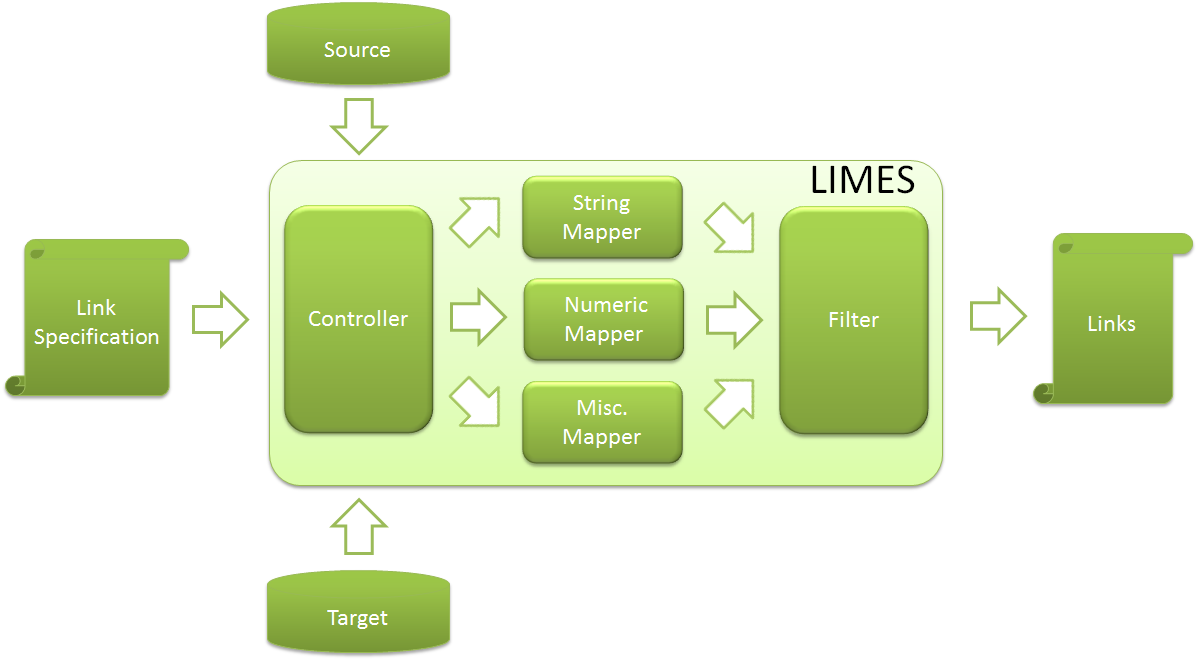
\includegraphics[width = 0.95\textwidth]{images/workflow.png}
			\caption{General Workflow of LIMES}
			\label{fig:workflow}
		\end{figure}

The general workflow implemented by the LIMES framework is depicted in Figure~\ref{fig:workflow}.
Given the source $S$, the target $T$ and a link specification, LIMES first separates the different data types to merge. 
Strings are processed by using suffix-, prefix- and position filtering in the string mapper.
Numeric values (and all values that can be mapped efficiently to a vector space) are mapped to a metric space and processed by the HYPPO algorithm.
All other values are mapped by using the miscellaneous mapper.
The results of all mappers processing are filtered and merged by using time-efficient set and filtering operations.

The advantages of LIMES' approach are manifold. 
First, it implements \textbf{highly time-optimized} mappers, making it a complexity class faster than other Link Discovery Frameworks. Thus, the larger the problem, the faster LIMES is w.r.t. other Link Discovery Frameworks. In addition, \textbf{LIMES is guaranteed to lead to exactly the same matching as a brute force approach while at the same time reducing significantly the number of comparisons}. In addition, LIMES supports a \textbf{large number of input and output formats} and can be extended very easily to fit new algorithms , new datatypes, new preprocessing functions and others thank to its modular architecture displayed in Figure \ref{fig:architecture}.

\begin{figure}[ht!]
			\centering
			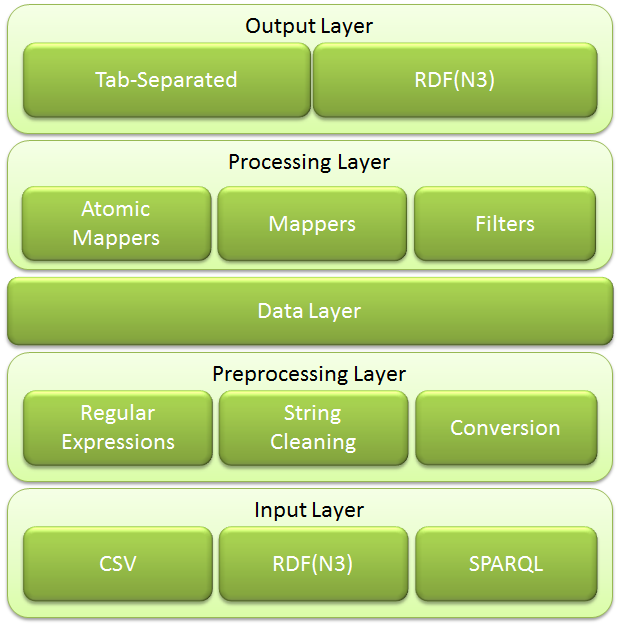
\includegraphics[width = 0.6\textwidth]{images/architecture.png}
			\caption{Architecture of LIMES}
			\label{fig:architecture}
		\end{figure}
		
In general, LIMES can be used to set links between two data sources, e.g., a novel data source created by a data publisher and existing data source such as DBpedia\footnote{\url{http://dbpedia.org}}. This functionality can also be used to detect duplicates within one data source for knowledge curation. The only requirement to carry out these tasks is a simple XML-based configuration file. The purpose of this manual is to explicate the LIMES Configuration Language (LCL) that underlies these configuration files, so as allow users to generate their own configurations. An online version of LIMES is available online at $\texttt{http://limes.aksw.org}$.

\section{Components of a LIMES Configuration File}
A LIMES configuration file consists of ten parts, of which some are optional:
\begin{enumerate}
\item Metadata
\item Prefixes
\item Source data source
\item Target data source
\item Metric for similarity measurement
\item Acceptance condition
\item Review condition 
\item Execution mode (optional)
\item Granularity (optional)
\item Output format
\end{enumerate}
In the following, we will explicate these components by showing successively how LIMES can be configured to compute a mapping between diseases contained in Bio2RDF and LinkedCT.
\subsection{Metadata}
The metadata for a LIMES config file always consists of the following bits of XML:

\begin{ttfamily}
\begin{lstlisting}[language=XML,basicstyle=\scriptsize,numberstyle=\tiny]
<?xml version="1.0" encoding="UTF-8"?>
<!DOCTYPE LIMES SYSTEM "limes.dtd">
<LIMES>
\end{lstlisting}
\end{ttfamily}

\subsection{Prefixes}
Defining a prefix in a LIMES file demands setting two values: the namespace that will be addresses by the prefix and the prefix per se, as shown below. 
\begin{ttfamily}
\begin{lstlisting}[language=XML,basicstyle=\scriptsize,numberstyle=\tiny]
<PREFIX>
		<NAMESPACE>http://www.w3.org/1999/02/22-rdf-syntax-ns#</NAMESPACE>
		<LABEL>rdf</LABEL>
</PREFIX>
\end{lstlisting}
\end{ttfamily}
Here, we set the prefix \texttt{rdf} to correspond to \texttt{http://www.w3.org/1999/02/22-rdf-syntax-ns\#}. A LIMES link specification can contain as many prefixes as required.

\subsection{Source Data Source}
LIMES computes links between items contained in two Linked Data sources dubbed source and target. An example of a configuration for a source data source is shown below.
\begin{ttfamily}
\begin{lstlisting}[language=XML,basicstyle=\scriptsize,numberstyle=\tiny]
<SOURCE>
	<ID>mesh</ID>
	<ENDPOINT>http://mesh.bio2rdf.org/sparql</ENDPOINT>
	<VAR>?y</VAR>
	<PAGESIZE>5000</PAGESIZE>
	<RESTRICTION>?y rdf:type meshr:Concept</RESTRICTION>
	<PROPERTY>dc:title</PROPERTY>
	<TYPE>sparql</TYPE>
</SOURCE>
\end{lstlisting}
\end{ttfamily}

Six properties need to be set. 
\begin{enumerate}
\item Each data source must be given an ID via the tag \texttt{ID}.
\item The SPARQL endpoint of the data source needs to be explicated via the \texttt{ENDPOINT} tag. In case local files (CSV, N3, TURTLE, etc.) are to be linked, \texttt{ENDPOINT} should be set to the absolute path of the file containing the data to link.
\item The variable associated with this endpoint must be specified. This is done by setting the \texttt{VAR} tag. This variable is used later when specifying the metric used to compare the entities retrieved from the source and target endpoints.
\item The fourth property is set via the \texttt{PAGESIZE} tag. This property must be set to the maximal number of triples returned by the SPARQL endpoint to address. For example, the DBpedia endpoint at \url{http://dbpedia.org/sparql} returns a maximum of 1000 triples for each query. LIMES' SPARQL module can still retrieve all relevant instances for the mapping if given this value. If the SPARQL endpoint does not limit the number of triple it returns or if the input is a file, the value of \texttt{PAGESIZE} should be set to -1. 
\item The restrictions of the data to retrieved can be set via the \texttt{RESTRICTION} tag. This tag allows to limit the entries that are retrieved the LIMES' query module. In this particular example, we only instances of MESH concepts. 
\item The \texttt{PROPERTY} tag allows to specify the properties that will be used during the linking. It is important to note that the property tagcan also be used to specify the preprocessing on the input data. For example, setting \texttt{rdfs:label AS nolang}, one can ensure that the language tags get removed from each \texttt{rdfs:label} before it is written in the cache. Pre-processing functions can be piped into one another by using \texttt{->}. For example, \texttt{rdfs:label AS nolang->lowercase} will compute \texttt{lowercase(nolang(rdfs:label))}.
\end{enumerate}

 The pre-processing functions include: 
\begin{itemize}
\item \texttt{nolang} for removing language tags, 
\item \texttt{lowercase} for converting the input string into lower case,  
\item \texttt{uppercase} for converting the input string into upper case, 
\item \texttt{number} for ensuring that only the numeric characters, ``.'' and ``,'' are contained in the input string,
\item \texttt{replace(String a,String b)} for replacing each occurrence of \texttt{a} with \texttt{b},
\item \texttt{cleaniri} for removing all the prefixes from IRIs,
\item \texttt{celsius} for converting Fahrenheit to Celsius,
\item \texttt{fahrenheit} for converting Celsius to Fahrenheit.
\end{itemize}

Sometimes, generating the right link specification might either require merging property values (for example, the \texttt{dc:title} and \texttt{foaf:name} of MESH concepts) or splitting property values (for example, comparing the label and \texttt{foaf:homepage} of source instances and the \texttt{foaf:homepage} of target instances as well as \texttt{foaf:homepage AS cleaniri} of the target instances with the \texttt{rdfs:label} of target instances. To enable this goal, LIMES provides the \texttt{RENAME} operator which simply store either the values of a property or the results of a preprocessing into a different property field. For example, \texttt{foaf:homepage AS cleaniri RENAME label} would stored the homepage of a object without all the prefixes in the name property. The user could then access this value during the specification of the similarity measure for comparing sources and target instances. Note that the same property value can be used several times. Thus, the following specification fragment is valid and leads to the the \texttt{dc:title} and \texttt{foaf:name} of individuals)  of MESH concepts being first cast down to the lowercase and then merged to a single property.

\begin{ttfamily}
\begin{lstlisting}[language=XML,basicstyle=\scriptsize,numberstyle=\tiny]
<SOURCE>
	<ID>mesh</ID>
	<ENDPOINT>http://mesh.bio2rdf.org/sparql</ENDPOINT>
	<VAR>?y</VAR>
	<PAGESIZE>5000</PAGESIZE>
	<RESTRICTION>?y rdf:type meshr:Concept</RESTRICTION>
	<PROPERTY>dc:title AS lowercase RENAME name</PROPERTY>
	<PROPERTY>foaf:name AS lowercase RENAME name</PROPERTY>
	<TYPE>sparql</TYPE>
</SOURCE>
\end{lstlisting}
\end{ttfamily}

In addition, the following allows splitting the values of \texttt{foaf:homepage} into the property values \texttt{name} and \texttt{homepage}.

\begin{ttfamily}
\begin{lstlisting}[language=XML,basicstyle=\scriptsize,numberstyle=\tiny]
<SOURCE>
	<ID>mesh</ID>
	<ENDPOINT>http://mesh.bio2rdf.org/sparql</ENDPOINT>
	<VAR>?y</VAR>
	<PAGESIZE>5000</PAGESIZE>
	<RESTRICTION>?y rdf:type meshr:Concept</RESTRICTION>
	<PROPERTY>foaf:homepage AS lowercase RENAME homepage</PROPERTY>
	<PROPERTY>foaf:homepage AS cleaniri->lowercase RENAME name</PROPERTY>
	<TYPE>sparql</TYPE>
</SOURCE>
\end{lstlisting}
\end{ttfamily}

In addition, a source type can be set via \texttt{TYPE}. The default type is set to \texttt{SPARQL} (for a SPARQL endpoint) but LIMES also supports reading files directly from the harddrive. The supported data formats are
\begin{itemize}
\item \texttt{CSV}: Character-separated file can be loaded directly into LIMES. Note that the separation character is set to \texttt{TAB} as a default. The user can alter this setting programmatically. 
\item \texttt{N3} (which also reads \texttt{NT} files) reads files in the \texttt{N3} language.
\item \texttt{N-TRIPLE} reads files in W3C's core N-Triples format.\footnote{\url{http://www.w3.org/TR/rdf-testcases/\#ntriples}}
\item  \texttt{TURTLE} allows reading files in the \texttt{Turtle} syntax.\footnote{\url{http://www.w3.org/TR/turtle/}}
\end{itemize}
Consequently, if you want to download data from a SPARQL endpoint, there is no need to set the \texttt{<TYPE>} tag. 
If instead you want to read the source (or target) data from a file, the \texttt{<ENDPOINT>} tag should contain the path to the file to read, e.g. \texttt{<ENDPOINT>C:/Files/dbpedia.nt</ENDPOINT>}
In addition, the \texttt{<TYPE>} tag then needs to be set, for example by writing \texttt{<TYPE>NT</TYPE>}.
\subsection{Target Data Source}
Configuring the target data source is very similar to configuring the source data source. The only difference lies in the beginning tag, i.e., \texttt{TARGET} instead of \texttt{SOURCE}. In the example shown below, we retrieve the \texttt{condition\_name} of a condition from LinkedCT. We do no set the type of the source. Thus, LIMES supposes it is a SPARQL endpoint.

\begin{ttfamily}
\begin{lstlisting}[language=XML,basicstyle=\scriptsize,numberstyle=\tiny]
<TARGET>
	<ID>linkedct</ID>
	<ENDPOINT>http://data.linkedct.org/sparql</ENDPOINT>
	<VAR>?x</VAR>
	<PAGESIZE>5000</PAGESIZE>
	<RESTRICTION>?x rdf:type linkedct:condition</RESTRICTION>
	<PROPERTY>linkedct:condition_name</PROPERTY>
</TARGET>
\end{lstlisting}
\end{ttfamily}

\subsection{Metric Expression for Similarity Measurement}
One of the core improvements of the newest LIMES kernels is the provision of a highly flexible language for the specification of complex metrics for linking (set by using the \texttt{METRIC} tag as exemplified below).

\begin{ttfamily}
\begin{lstlisting}[language=XML,basicstyle=\scriptsize,numberstyle=\tiny]
<METRIC>
trigrams(y.dc:title, x.linkedct:condition_name)
</METRIC>
\end{lstlisting}
\end{ttfamily}

In this example, we use the Trigrams metric to compare the \texttt{dc:title} of the instances retrieved from the source data source, with which the variable \texttt{y} is associated, with the \texttt{linkedct:}\\\texttt{condition\_name} of the instances retrieved from the target data source, with which the variable \texttt{x} is associated. While such simple metrics can be used in many cases, complex metrics are necessary in complex linking cases. LIMES includes a formal grammar for specifying complex configurations of arbitrary complexity. For this purpose, two categories of binary operations are supported: Metric operations and boolean operations.

\textbf{Metric operations} allow to combine metric values. They include the operators \texttt{MIN}, \texttt{MAX}, \texttt{ADD} and \texttt{MULT}, e.g. as follows:

\begin{ttfamily}
\begin{lstlisting}[language=XML,basicstyle=\scriptsize,numberstyle=\tiny]
MAX(trigrams(x.rdfs:label,y.dc:title),euclidean(x.lat|long, y.latitude|longitude)).
\end{lstlisting}
\end{ttfamily}

This specification computes the maximum of (1) the trigram similarity of x's \texttt{rdfs:label} and y's \texttt{dc:title} and (2) the 2-dimension euclidean distance of x's \texttt{lat} and \texttt{long} mit y's \texttt{latitude} and \texttt{longitude}, i.e., 

$\sqrt{(x.lat- y.latitude)^2 + (x.long - y.longitude)^2}$. 

Note that euclidean supports arbitrarily many dimensions. In addition, note that \texttt{ADD} allows to define weighted sums as follows:

\begin{ttfamily}
\begin{lstlisting}[language=XML,basicstyle=\scriptsize,numberstyle=\tiny]
ADD(0.3*trigrams(x.rdfs:label,y.dc:title), 
    0.7*euclidean(x.lat|x.long, y.latitude|y.longitude)).
\end{lstlisting}
\end{ttfamily}

\textbf{Boolean operations} allow to combine and filter the results of metric operations and include \texttt{AND}, \texttt{OR}, \texttt{DIFF}, e.g. as follows:

\begin{ttfamily}
\begin{lstlisting}[language=XML,basicstyle=\scriptsize,numberstyle=\tiny]
AND(trigrams(x.rdfs:label,y.dc:title)|0.9,
    euclidean(x.lat|x.long, y.latitude|y.longitude)|0.7).
\end{lstlisting}
\end{ttfamily}

This specification returns all links such that (1) the trigram similarity of x's \texttt{rdfs:label} and y's \texttt{dc:title} is greater or equal to 0.9 and (2) the 2-dimension euclidean distance of x's \texttt{lat} and \texttt{long} mit y's \texttt{latitude} and \texttt{longitude} is greater or equal to 0.7.

The current version of LIMES supports the string metrics 
\begin{itemize}
\item \texttt{Trigrams}
\item \texttt{Cosine}
\item \texttt{Jaccard} and 
\item \texttt{Levenshtein}.
\end{itemize}
\texttt{Overlap}, \texttt{Jaro}, \texttt{Jaro-Winkler} as well as \texttt{Monge-Elkan} are currently being added.
In addition it supports comparing numeric vectors by using the 
\begin{itemize}
\item \texttt{Euclidean} metric as well as 
\item the \texttt{Orthodromic} distance.
\end{itemize}
The similarity between polygons can be measured by using the 
\begin{itemize}
\item \texttt{Hausdorff} distance as well as the
\item \texttt{SymmetricHausdorff} distance.
\end{itemize}
More complex distance measures are being added.
%
%\subsection{Number of exemplars}
%The user can choose to set the number of exemplars to be used by LIMES manually. This setting can be carried out as shown below.
%\begin{verbatim}
%<EXEMPLARS> 70 </EXEMPLARS>
%\end{verbatim}
%In this example, the number of exemplars is set to 70. It is important to notice that this setting is optional. If not set, LIMES uses the value  $\lfloor{\sqrt{|T|}}\rfloor$ for the number of exemplars, where $T$ is the target knowledge source for the matching task.

\subsection{Acceptance Condition}
Setting the acceptance condition basically consists of setting the value for the threshold above which links are considered to be valid and not to required further curation. This can be carried out as exemplified below.
\begin{ttfamily}
\begin{lstlisting}[language=XML,basicstyle=\scriptsize,numberstyle=\tiny]
<ACCEPTANCE>
	<THRESHOLD>0.98</THRESHOLD>
	<FILE>accepted.nt</FILE>
	<RELATION>owl:sameAs</RELATION>
</ACCEPTANCE>
\end{lstlisting}
\end{ttfamily}

By using the \verb#THRESHOLD# tag, the user can set the value for the metric value above which two instances are considered to be linked via the relation specified by using the tag \verb#RELATION#, i.e., \verb#owl:sameAs# in our example. Setting the tag \verb#FILE# allows to specify where the links should be written. Currently, LIMES produces output files in the N3 format.

Future versions of LIMES will allow to write the output to other streams and in other data formats.

\subsection{Review Condition}
Setting the condition upon which links must be reviewed manually is very similar to setting the acceptance condition as shown below.

\begin{ttfamily}
\begin{lstlisting}[language=XML,basicstyle=\scriptsize,numberstyle=\tiny]
<REVIEW>
	<THRESHOLD>0.95</THRESHOLD>
	<FILE>reviewme.nt</FILE>
	<RELATION>owl:sameAs</RELATION>
</REVIEW>
\end{lstlisting}
\end{ttfamily}

All instances that have a similarity between the threshold set in \texttt{REVIEW} (0.95 in our example) and the threshold set in \texttt{ACCEPTANCE} (0.98 in our example) will be written in the review file and linked via the relation set in \texttt{REVIEW}. 
 
The LIMES configuration file should be concluded with \texttt{</LIMES>}

\subsection{Execution Mode (optional)}

The user can choose between the executions modes \texttt{SIMPLE} and \texttt{FILTER} to tune LIMES' runtime. 
\begin{ttfamily}
\begin{lstlisting}[language=XML,basicstyle=\scriptsize,numberstyle=\tiny]
<EXECUTION>SIMPLE</EXECUTION>.
\end{lstlisting}
\end{ttfamily}

\subsection{Granularity (optional)}

The user can choose positive integers to set the granularity of HYPPO, HR3 or ORCHID by setting

\begin{ttfamily}
\begin{lstlisting}[language=XML,basicstyle=\scriptsize,numberstyle=\tiny]
<GRANULARITY>2</GRANULARITY>.
\end{lstlisting}
\end{ttfamily}

\subsection{Output Format}
The user can choose between TAB and N3 as output format by setting

\begin{ttfamily}
\begin{lstlisting}[language=XML,basicstyle=\scriptsize,numberstyle=\tiny]
<OUTPUT>N3</OUTPUT>
\end{lstlisting}
\end{ttfamily}


\section{Example of a Configuration File}
The following shows the whole configuration file for LIMES explicated in the sections above.

\begin{ttfamily}
\begin{lstlisting}[language=XML,basicstyle=\scriptsize,numbers=left,numberstyle=\tiny]
<?xml version="1.0" encoding="UTF-8"?>
<!DOCTYPE LIMES SYSTEM "limes.dtd">
<LIMES>
	<PREFIX>
		<NAMESPACE>http://www.w3.org/1999/02/22-rdf-syntax-ns#</NAMESPACE>
		<LABEL>rdf</LABEL></PREFIX>
	<PREFIX>
		<NAMESPACE>http://www.w3.org/2000/01/rdf-schema#</NAMESPACE>
		<LABEL>rdfs</LABEL></PREFIX>
	<PREFIX>
		<NAMESPACE>http://www.w3.org/2002/07/owl#</NAMESPACE>
		<LABEL>owl</LABEL></PREFIX>
	<PREFIX>
		<NAMESPACE>http://data.linkedct.org/resource/linkedct/</NAMESPACE>
		<LABEL>linkedct</LABEL></PREFIX>
	<PREFIX>
		<NAMESPACE>http://purl.org/dc/elements/1.1/</NAMESPACE>
		<LABEL>dc</LABEL></PREFIX>
	<PREFIX>
		<NAMESPACE>http://bio2rdf.org/ns/mesh#</NAMESPACE>
		<LABEL>meshr</LABEL></PREFIX>
		
  <SOURCE>
		<ID>mesh</ID>
		<ENDPOINT>http://mesh.bio2rdf.org/sparql</ENDPOINT>
		<VAR>?y</VAR>
		<PAGESIZE>5000</PAGESIZE>
		<RESTRICTION>?y rdf:type meshr:Concept</RESTRICTION>
		<PROPERTY>dc:title</PROPERTY>
	</SOURCE>
		
	<TARGET>
		<ID>linkedct</ID>
		<ENDPOINT>http://data.linkedct.org/sparql</ENDPOINT>
		<VAR>?x</VAR>
		<PAGESIZE>5000</PAGESIZE>
		<RESTRICTION>?x rdf:type linkedct:condition</RESTRICTION>
		<PROPERTY>linkedct:condition_name</PROPERTY>
	</TARGET>	

	<METRIC>
	 MAX(trigrams(y.dc:title, x.linkedct:condition_name), 
	     cosine(y.dc:title, x.linkedct:name))
	</METRIC>

	<ACCEPTANCE>
		<THRESHOLD>0.98</THRESHOLD>
		<FILE>accepted.txt</FILE>
		<RELATION>owl:sameAs</RELATION>
	</ACCEPTANCE>
	<REVIEW>
		<THRESHOLD>0.95</THRESHOLD>
		<FILE>reviewme.txt</FILE>
		<RELATION>owl:sameAs</RELATION>
	</REVIEW>
</LIMES>
\end{lstlisting}
\end{ttfamily}


\section{The LIMES Distribution}
\subsection{Content}
The LIMES distribution in its current version 0.5.RC1 contains the files
\begin{itemize}
\item \texttt{LIMES.jar}, which implements our framework,
\item \texttt{limes.dtd}, the data type definition for LIMES configuration files and
\item \texttt{user\_manual.pdf}, this file. 
\end{itemize}
In addition, it contains the folders
\begin{itemize}
\item \texttt{lib}, which contains all the libraries necessary to run our framework and
\item \texttt{examples}, which contains examples of configuration files.
\end{itemize}
\subsection{Running the Framework} 
Once the configuration file (dubbed \texttt{config.xml} in this manual) has been written, the last step consists of actually running the LIMES framework. For this purpose, simply run

\texttt{java -jar LIMES.jar config.xml}. 

In case your system runs out of memory, please use the \texttt{-Xmx} option to allocate more memory to the Java Virtual Machine. Please ensure that the Data Type Definition file for LIMES, \texttt{limes.dtd}, is in the same folder as the \texttt{LIMES.jar} and everything should run just fine. Enjoy.

\section{Support Information}
For support, please contact:

Axel-Cyrille Ngonga Ngomo

Johanisgasse 26

Room 5-22

04103 Leipzig

\verb#ngonga@informatik.uni-leipzig.de#

\section{License and Warranty Information}
LIMES is free to use for non-commercial purposes.
For any kind of commercial use, please contact us.
Also note that LIMES is distributed without any warranty of any type.

\section{Known Issues}

None.

\section{Change log}
\subsection{Version 0.6RC3}
\begin{itemize}
\item Added support for geo-spatial similarity function based on Hausdorff distance
\item Added support for geo-spatial similarity function based on symmetric Hausdorff distance
\item Added support for orthodromic distance
\item Implemented ORCHID for time-efficient linking of geo-spatial resources
\item Added support for exact matches
\end{itemize}


\subsection{Version 0.6RC2}
\begin{itemize}
\item Time-efficient self-configuration (genetic, linear, boolean)
\item Can now read use most RDF serialization formats (RDF/XML, N3, NT, TTL) as input
\end{itemize}

\subsection{Version 0.6RC1}
\begin{itemize}
\item Kernel update
\item HR3 algorithm for vector space. Default granularity is now 4.
\item Update for data readers and writers.
\item Genetic Learning
\end{itemize}

\subsection{Version 0.5RC1}
\begin{itemize}
\item Kernel change, more than 4 orders of magnitude faster
\item HYPPO algorithm for vector spaces
\item Fast prefix, suffix and position filtering for strings
\item Support for more metrics
\end{itemize}
\subsection{Version 0.4.1}
\begin{itemize}
\item Added support for data source type (tab-separated vectors)
\item Added factory for query modules
\end{itemize}

\subsection{Version 0.4}
\begin{itemize}
\item Added support for data source type (Sparql, CSV)
\item Added hybrid cache
\item Implemented CSV reader
\item Faster organizer 
\end{itemize}
>>>>>>> .r778
\end{comment}
\end{document}